\documentclass[conference]{IEEEtran}
\IEEEoverridecommandlockouts
\usepackage{cite}
\usepackage{amsmath,amssymb,amsfonts}
\usepackage{graphicx}
\usepackage{textcomp}
\usepackage{xcolor}
\usepackage{booktabs}
\usepackage{array}
\usepackage{enumitem}
\usepackage{url}
\usepackage{tikz}
\usetikzlibrary{arrows.meta,positioning,shapes.geometric,calc,fit,backgrounds,decorations.pathreplacing}
\usepackage{pgfplots}
\pgfplotsset{compat=1.16}
\newcolumntype{P}[1]{>{\raggedright\arraybackslash}p{#1}}
% Placeholder marker (only shown if a figure file is missing)
\newcommand{\todo}[1]{\textcolor{red}{[#1]}}

% TikZ styles for diagrams (same as the project report)
\tikzset{
  blk/.style={draw, rounded corners=2pt, align=center, minimum height=13mm,
              text width=25mm, font=\footnotesize, fill=gray!8},
  arr/.style={-{Stealth[length=2.2mm]}, thick}
}

% Author block: equal-width boxes, 3 + 2 centred
\newcommand{\authorbox}[2]{%
  \parbox[t]{0.325\textwidth}{\centering
    {\normalsize #1}\\[1pt]
    {\footnotesize\itshape Dept. of Computer Science\\and Engineering\\
    Amrita School of Computing, Bengaluru\\
    Amrita Vishwa Vidyapeetham, India\\
    Bengaluru, India}\\[1pt]
    {\footnotesize #2}}}

\begin{document}

\title{FireVLM: Parameter-Efficient Fine-Tuning of a Vision-Language Model for Wildfire Visual Question Answering}

\author{%
\authorbox{Rishab Ramesh Nair}{bl.en.u4aie23126@bl.students.amrita.edu}%
\hfill
\authorbox{Praanesh Balakrishnan Nair}{bl.en.u4aie23123@bl.students.amrita.edu}%
\hfill
\authorbox{Sanjushree Rajan}{bl.en.u4aie23130@bl.students.amrita.edu}\\[8pt]
\authorbox{Varun Adhitya G B}{bl.en.u4aie23135@bl.students.amrita.edu}%
\hspace{0.05\textwidth}%
\authorbox{Rimjhim Padam Singh}{ps\_rimjhim@blr.amrita.edu}%
}

\maketitle

\begin{abstract}
Visual Question Answering (VQA) is being developed to allow a natural-language question to be asked of an active fire scene by using a pair of visible (RGB) and radiometric (thermal) inputs. This work examines the WildFireVQA dataset and the parameter-efficient adaptation of vision-language models on the Sycan Marsh subset (738 image pairs, 34 questions per image pair, 25,092 question--answer pairs). Two types of adaptation are explored: a frozen pretrained Qwen2.5-VL-3B-Instruct model using in-context prompting (0--10 demonstrations; 200 query samples), and compact models with a frozen CLIP ViT-B/32 encoder, trainable projectors, and a language model fine-tuned using QLoRA with 4-bit quantization over multiple adapter ranks and target modules. The frozen baseline reaches an accuracy of 28.00\% with ten demonstrations and 15.00\% with zero. Fine-tuned Qwen2-1.5B models, evaluated on 2,482 test queries, reach 84.13\% to 86.62\% exact match with 5.8 to 23.2 million trainable parameters. The configurations that use query, key, value, and output attention projections at rank 4 and rank 8 are within the sampling uncertainty of each other (86.62\% and 86.30\%), while larger all-linear adapters or higher ranks do not improve accuracy. The Llama-3.2-1B backbone reaches 85.46\% to 88.48\%. The results suggest that compact budgets of attention-only adapters are adequate for domain-specific VQA on fire scenes.
\end{abstract}

\begin{IEEEkeywords}
wildfire monitoring, visual question answering, thermal imaging,
vision-language models, parameter-efficient fine-tuning, LoRA
\end{IEEEkeywords}

\section{Introduction}

\subsection{Introduction to Wildfire Visual Question Answering}

Wildfires can cause extensive damage to ecological systems, people and property. Visible spectrum (RGB) and radiometric thermal imagery is captured over active fire areas using aerial surveillance platforms, including unmanned aerial vehicles (UAVs). Situation awareness generally relies on manual analysis of these sensor streams, which is time-intensive and susceptible to error.

In this project, we aim to research how to adapt vision-language models with fewer parameters in the field of Wildfire Visual Question Answering. We benchmark two adaptation regimes: (i) an in-context learning baseline that uses a frozen pretrained Qwen2.5-VL-3B-Instruct model with zero to ten demonstrations to prompt the model \cite{brown2020,bai2025} and (ii) a modular VL architecture with a frozen ViT-B/32 vision encoder \cite{radford2021} and dual trainable projection layers, along with a 4-bit quantized language model (Qwen2-1.5B \cite{qwen2,mithan} or Llama-3.2-1B \cite{llama32}) fine-tuned using Low-Rank Adaptation (LoRA/QLoRA) \cite{dettmers2023,hu2022}.

\subsection{Motivation}

Emergency response agencies need to extract information quickly and accurately from aerial fire feeds. However, tuning large-scale, multi-billion-parameter foundation models requires high-memory GPUs, often unavailable to regional monitoring centers and research labs. Low-rank adapters and 4-bit weight quantization significantly reduce training and memory consumption and are highly parameter-efficient fine-tuning methods. The extent of adapter capacity required for multimodal disaster question answering, however, is still an open question. This work investigates the effects of adapter rank and layer positions on task accuracy and parameter count.

\subsection{Problem Statement}

Given an RGB and a radiometric thermal image, along with a natural-language question, produce a concise, correct response while optimizing trainable parameters and operating within the memory restrictions of a single commodity GPU.

\subsection{Objectives}

\begin{itemize}[leftmargin=*, itemsep=1pt, topsep=2pt, parsep=0pt]
  \item Create an audited image split of the Sycan Marsh subset of WildFireVQA with no file overlap with the Flame3 subset.
  \item Evaluate a frozen pretrained vision-language model on 0-shot to 10-shot in-context demonstrations to measure the base performance of the model on the output format and zero-shot reasoning in the absence of finetuning.
  \item Build a parameter-efficient vision-language model based on a frozen CLIP vision encoder and two trainable modality projectors along with 4-bit quantized language models (Qwen2-1.5B and Llama-3.2-1B).
  \item Compare placement of the adapters (attention projections and all linear projections) and rank sweep to find the least parameter budget needed for visual question answering of fire scenes.
\end{itemize}

\section{Literature Survey}

\subsection{Parameter-Efficient Fine-Tuning for Vision-Language Models}

\subsubsection{The Evolution Beyond Transformers}

As VLMs scale to billions of parameters, parameter-efficient fine-tuning (PEFT) has become critical. Recently, a survey was published that focuses on PEFT methods for post-Transformer architectures, such as Mamba-based state-space models, RWKV recurrent models and hybrid models that incorporate attention with linear-complexity architectures~\cite{peft2024survey}. PEFT methods are divided into 4 families: (1) Additive methods: add new trainable modules (adapters, prompt tuning, prefix tuning); (2) Selective methods: update only a subset of the parameters -- either update bias terms (BitFit) or learn sparse masks (diff pruning); (3) Reparameterization methods: decompose the weight updates into low-rank matrices (LoRA); (4) Hybrid methods: use multiple strategies (e.g., MAM Adapter combines LoRA with parallel FF adapters).

Low-rank adaptation (LoRA)~\cite{hu2022} learns the weight updates as low-rank matrices, achieving a significant decrease in the number of parameters to be trained while maintaining a high degree of expressiveness. LoRA is an approach that fixes the weight matrix $W \in \mathbb{R}^{d \times k}$, and trains an additive update to it: $\Delta W \leftarrow BA$ with $B \in \mathbb{R}^{d \times r}$ and $A \in \mathbb{R}^{r \times k}$, where the rank $r \ll \min(d,k)$. This decreases the number of trainable parameters from $dk$ to $r(d+k)$. LoRA's main idea is that task specific adaption frequently occurs in a low-dimensional subspace of the space of parameters, so you can use a low-rank update. Ranks as low as 1--8 are already found to perform near the performance of full fine-tuning on natural language tasks, but may require a higher rank for vision-language tasks (4--16) because of the difficulty of cross-modal reasoning.

\subsection{Vision-Language Models in Remote Sensing and Disaster Response}

\subsubsection{Wildfire Visual Question Answering}

The WildFireVQA benchmark~\cite{wildfirevqa} fills an important void in disaster response VLMs. The dataset is made up of 3 prescribed burns (Sycan Marsh, Willamette, Shoetank) with 6,097 sets of RGB-thermal images taken by the FLAME~3 project~\cite{flame3} at Clemson University. The images are each accompanied by 34 questions organized into six categories: presence/detection (Is there fire?); counting (How many hotspots?); spatial reasoning (Where is the smoke compared to the flame?); understanding of the scene (What is the dominant vegetation?); temperature analysis (What is the maximum temperature?); and comparative reasoning (Which area is hotter?) This gives a total of 207,298 QAPs.

\subsection{Gap Analysis and Positioning}

While there has been tremendous progress for VLMs and PEFT, there are still a number of gaps that exist for wildfire VQA:
\begin{itemize}[leftmargin=*, itemsep=1pt, topsep=2pt, parsep=0pt]
    \item {Limited domain-specific benchmarks:} WildFireVQA is one of the first VQA benchmarks for radiometric thermal monitoring of wildfires, and includes three burn sites. Generalization to other types of fire (urban, industrial), to geographic regions and to other disaster scenarios (floods, hurricanes) is not investigated.
    \item {Insufficient thermal reasoning:} Current VLMs on RGB images don't work with radiometric thermal data. Knowing the physical units, characteristics of sensors, and thermal-visual correspondences are not part of general pretraining and is necessary for temperature-based reasoning.
    \item {Adapter capacity vs accuracy trade-offs:} adapter capacity (rank, layer placement) and task-specific accuracy for wildfire VQA are not well understood. Previous studies examined PEFT in natural-image applications, but fire imagery has different image properties (sparse fire scenes, thermal modality, high image resolution) which may require a different adapter configuration.
    \item {Real-time deployment constraints:} Operational wildfire systems have to deliver answers within seconds to aid decision making during active wildfire events. Current benchmarks measure accuracy off-line, but do not consider the latency-accuracy-memory trade off in VLMs deployed on edge devices, such as an UAV onboard compute and mobile ground stations.
\end{itemize}
The above-identified approaches are summarised in Table~\ref{tab:related}.

\begin{table}[t]
\centering
\caption{Summary of related approaches and the gap addressed by this work}
\label{tab:related}
\footnotesize
\setlength{\tabcolsep}{3pt}
\begin{tabular}{@{}P{0.26\columnwidth}P{0.33\columnwidth}P{0.35\columnwidth}@{}}
\toprule
\textbf{Approach} & \textbf{Strength} & \textbf{Gap for wildfire VQA} \\
\midrule

Contrastive alignment \cite{ak2024aligning} & Improves vision-language embedding quality & Not specialized for thermal-RGB fusion \\
PEFT surveys \cite{peft2024survey} & Comprehensive adapter taxonomy & Adapter placement not studied on fire scenes \\
VL-PET \cite{vlpet2024} & Controls the size of adapter modifications & Encoder--decoder models; not studied on fire scenes \\
Remote sensing VLMs \cite{remotesensing2024} & Handles high-resolution imagery & Limited thermal reasoning, no fire focus \\
WildFireVQA benchmark \cite{wildfirevqa} & Safety-critical real-world task & Adapter capacity needed for the task not characterised \\
Molmo open models \cite{molmo2024} & Strong open baseline & Not adapted to thermal wildfire data \\
VisionCore spatial reasoning \cite{visioncore2024} & Enhanced localization & Not evaluated on disaster imagery \\
SynthVLM data synthesis \cite{synthvlm2024} & Reduces data cost with synthetic image--caption pairs & RGB only; cannot synthesise radiometric thermal data \\
\bottomrule
\end{tabular}
\end{table}

A considerable efficiency loss exists in the adapter when changing between different QLoRA settings, such as query/value, query/key/value/output, all linear layers, and ranks 4--16. This project aims to systematically compare the different configurations of QLoRA on WildFireVQA data set and determine the minimum budget required to attain comparable accuracy results. We will see a practical recipe for adapting compact models (1.5B parameters, 4-bit quantization) on free-tier hardware, to disaster imagery.

\section{System Design}

\subsection{High Level Design}

As shown in Fig.~\ref{fig:pipeline}, the fine-tuned vision-language model consists of three key components: a visual backbone, a language backbone, and a cross-modal module. Each sample contains an aerial visible RGB image and a radiometric thermal image from FLAME~3 together with a query from the WildFireVQA \cite{wildfirevqa,flame3}. Both images are scaled to $224\times224$ pixels. A frozen CLIP ViT-B/32 vision encoder \cite{radford2021} splits each image into $32\times32$ patches, giving a $7\times7$ grid and hence 49 patch tokens per image (98 visual tokens per sample). The 768-dimensional vision tokens are projected by two independent multilayer perceptron (MLP) projectors, one for the visible imagery and one for the thermal imagery, into the hidden dimension $d$ of the target language model (1536 for Qwen2-1.5B and 2048 for Llama-3.2-1B). Learned 1D modality type embeddings are added to differentiate the streams. The 98 visual tokens are placed as a prefix to the question in a chat-like prompt. The answer text gets then autoregressively generated using a 4-bit quantized decoder language model with adapters \cite{dettmers2023,hu2022}.

\begin{figure*}[!t]
  \centering
  \resizebox{\textwidth}{!}{%
  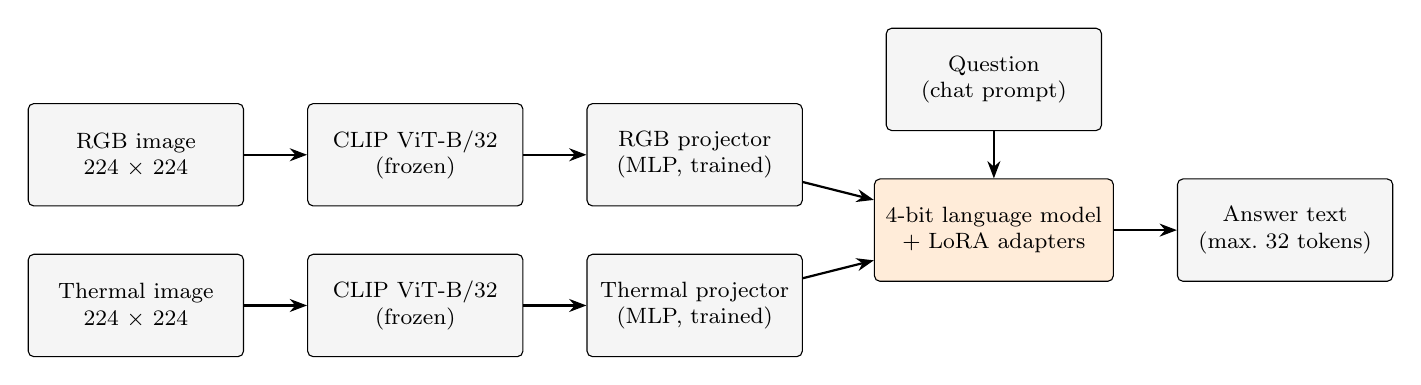
\begin{tikzpicture}[node distance=6mm and 8mm]
    \node[blk] (rgb) {RGB image\\$224\times224$};
    \node[blk, below=of rgb] (th) {Thermal image\\$224\times224$};
    \node[blk, right=of rgb] (c1) {CLIP ViT-B/32\\(frozen)};
    \node[blk, right=of th] (c2) {CLIP ViT-B/32\\(frozen)};
    \node[blk, right=of c1] (p1) {RGB projector\\(MLP, trained)};
    \node[blk, right=of c2] (p2) {Thermal projector\\(MLP, trained)};
    \node[blk, text width=28mm, fill=orange!15] (llm) at ($(p1)!0.5!(p2)+(38mm,0)$) {4-bit language model\\+ LoRA adapters};
    \node[blk, above=of llm] (q) {Question\\(chat prompt)};
    \node[blk, right=of llm] (ans) {Answer text\\(max.\ 32 tokens)};
    \draw[arr] (rgb) -- (c1);
    \draw[arr] (th) -- (c2);
    \draw[arr] (c1) -- (p1);
    \draw[arr] (c2) -- (p2);
    \draw[arr] (p1) -- (llm);
    \draw[arr] (p2) -- (llm);
    \draw[arr] (q) -- (llm);
    \draw[arr] (llm) -- (ans);
  \end{tikzpicture}}
  \caption{Architecture of the fine-tuned FireVLM models. Each projector outputs tokens of width $d$, the hidden width of the language model (1536 for Qwen2-1.5B, 2048 for Llama-3.2-1B).}
  \label{fig:pipeline}
\end{figure*}

\subsection{Low Level Design}

\subsubsection{Model Architectures}\label{sec:arch}

\textbf{CLIP ViT-B/32 (vision encoder).} The vision encoder is the image tower of CLIP \cite{radford2021}, a dual-encoder model originally trained contrastively on image--text pairs. A $224\times224$ input is split into $32\times32$ patches ($7\times7=49$ tokens), each linearly embedded to 768 dimensions with position embeddings added. A 12-layer, 12-head Transformer encoder with width 768 then processes the sequence through self-attention. The patch-level hidden states are used as visual tokens, while the text tower and contrastive head are not used. All CLIP weights remain frozen.

\textbf{Qwen2-1.5B (language backbone).} Qwen2 \cite{qwen2,mithan} is a decoder-only Transformer with 28 layers and hidden size 1536. It uses grouped-query attention (12 query heads sharing 2 key/value heads) to reduce the key--value cache, rotary position embeddings (RoPE), pre-RMSNorm, and a SwiGLU feed-forward block made of gate, up and down projections. Its seven linear modules ($q,k,v,o$, gate, up, down) are those targeted by the LoRA configurations in Table~\ref{tab:variants}. The base weights are quantized to 4-bit NF4 and frozen.

\textbf{Llama-3.2-1B (language backbone).} Llama-3.2-1B \cite{llama32} has a similar decoder-only design with 16 layers and hidden size 2048. It uses grouped-query attention (32 query and 8 key/value heads), RoPE, RMSNorm and SwiGLU feed-forward blocks. It exposes the same seven linear modules, so the same adapter placements are applied. Its wider hidden size means that the projectors emit 2048-dimensional tokens.

\textbf{Qwen2.5-VL-3B-Instruct (frozen baseline).} Unlike the two backbones above, the baseline \cite{bai2025} is a complete vision-language model: a native-resolution ViT encoder with window attention, an MLP merger that compresses visual tokens, and a Qwen2.5-3B language decoder. It receives images and text directly and is used only for in-context prompting, with no updates to the weights.

\subsubsection{Dataset and Data Splits}\label{sec:dataset}

The pipeline loads 207,306 rows of the WildFireVQA dataset from three prescribed burn sites: Shoetank (120,360 rows), Willamette (61,846 rows), and Sycan Marsh (25,092 rows). This study extracts the Sycan Marsh subset (25,092 rows) from the table. An initial pairing procedure maps each source annotation row to its canonical image pair based on the statistical information of radiometric temperature in the source annotation thermal TIFF files. A strict pairing audit is done to make certain that every question is paired to a different visible and thermal image pair, and that there are exactly 34 questions for each image pair: 738 visible and thermal image pairs; 622 Fire class, 116 No Fire class, 364 Sycan 2A and 374 Sycan 2D. The rows are deduplicated by both identifier and text, and assertions enforce that there are no duplicate questions in an image.

The Sycan Marsh subset, from 25,092 rows to 738 audited image pairs and three splits is shown in Fig.~\ref{fig:funnel}.

\begin{figure}[!t]
  \centering
  \resizebox{\columnwidth}{!}{%
  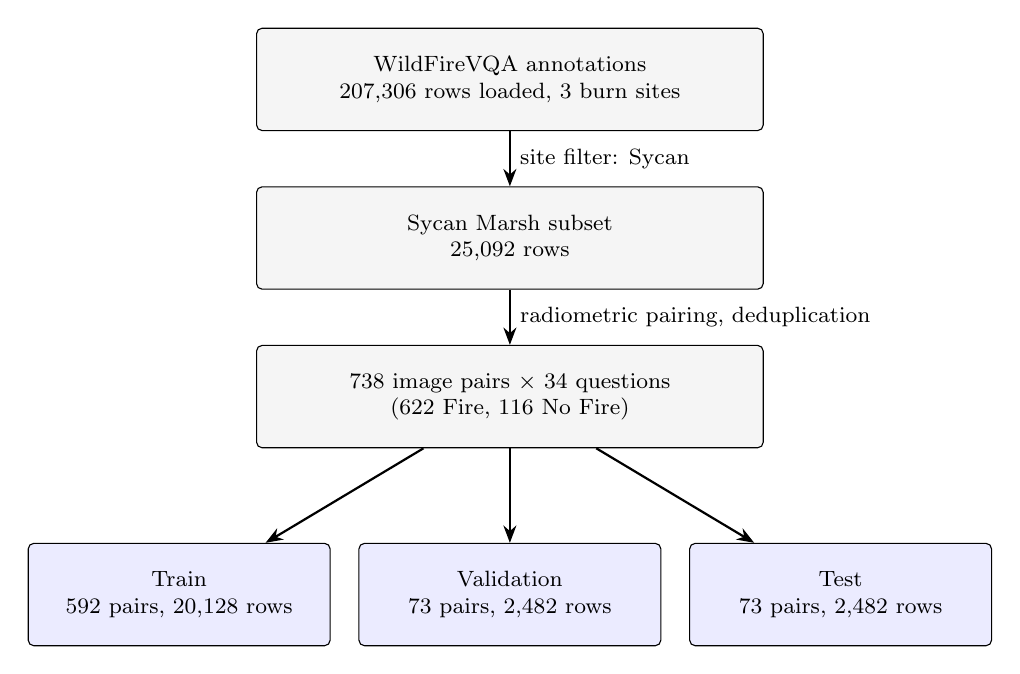
\begin{tikzpicture}[node distance=7mm]
    \node[blk, text width=62mm] (raw) {WildFireVQA annotations\\207,306 rows loaded, 3 burn sites};
    \node[blk, text width=62mm, below=of raw] (syc) {Sycan Marsh subset\\25,092 rows};
    \node[blk, text width=62mm, below=of syc] (pairs) {738 image pairs $\times$ 34 questions\\(622 Fire, 116 No Fire)};
    \node[blk, below=12mm of pairs, xshift=-42mm, text width=36mm, fill=blue!8] (tr) {Train\\592 pairs, 20,128 rows};
    \node[blk, below=12mm of pairs, text width=36mm, fill=blue!8] (va) {Validation\\73 pairs, 2,482 rows};
    \node[blk, below=12mm of pairs, xshift=42mm, text width=36mm, fill=blue!8] (te) {Test\\73 pairs, 2,482 rows};
    \draw[arr] (raw)--node[right, font=\footnotesize]{site filter: Sycan}(syc);
    \draw[arr] (syc)--node[right, font=\footnotesize]{radiometric pairing, deduplication}(pairs);
    \draw[arr] (pairs)--(tr); \draw[arr] (pairs)--(va); \draw[arr] (pairs)--(te);
  \end{tikzpicture}}
  \caption{From the raw WildFireVQA annotations to the image-grouped train, validation and test splits (all questions of an image stay in one split; seed 42).}
  \label{fig:funnel}
\end{figure}

Each image pair has 34 questions, all of which are contained within the image pair's partition. For the prompt, the options are omitted and the model is trained and generated to create free-form prose that is evaluated via string equality with the ground-truth answer, with whitespace stripped and lower-cased:
\begin{equation}
\text{EM}(\text{ref}, \text{pred}) = \mathbb{I}\bigl[\text{lower}(\text{strip}(\text{ref})) == \text{lower}(\text{strip}(\text{pred}))\bigr].
\end{equation}

\subsubsection{Experiment Configurations}

The summary of experimental configurations is given in Table~\ref{tab:variants} and in Fig.~\ref{fig:placement}. All 16 fine-tuning runs were trained, one for every configuration over both the Qwen2-1.5B and Llama-3.2-1B backbones. Low rank adapters are applied to attention projections (query $q$, key $k$, value $v$, output $o$) or all linear projections across attention and feedforward MLP blocks, including the gate, up and down projections. The design of the adapter focuses on the efficiency of parameters: to obtain high task accuracy with the fewest parameter additions. The distribution of rank sweeps across configurations was determined by time constraints and initial results of the previous experiments. In all fine-tuned models, the vision encoder is not updated during training, but only the two projectors and modality embeddings.

\begin{figure}[!t]
  \centering
  \resizebox{\columnwidth}{!}{%
  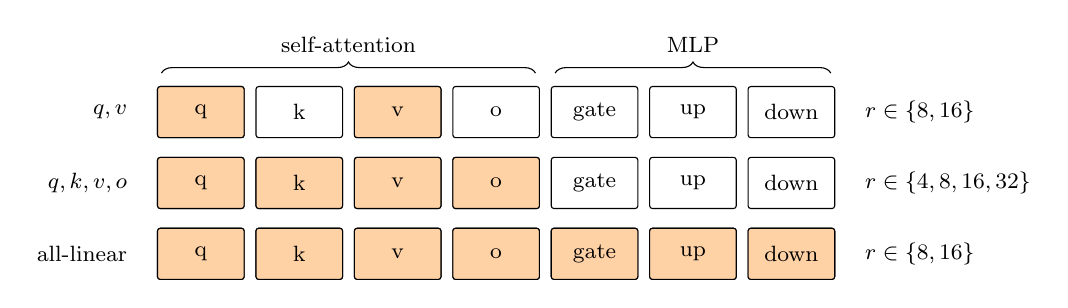
\begin{tikzpicture}[x=1.25cm, y=0.9cm, every node/.style={font=\footnotesize},
      mod/.style={draw, minimum width=1.1cm, minimum height=0.65cm, rounded corners=1pt},
      on/.style={mod, fill=orange!35}]
    \foreach \m [count=\i] in {q,k,v,o,gate,up,down}{
      \foreach \r in {0,-1,-2}{ \node[mod] at (\i,\r) {\m}; } }
    % adapted modules
    \foreach \i/\m in {1/q,3/v}{ \node[on] at (\i,0) {\m}; }
    \foreach \i/\m in {1/q,2/k,3/v,4/o}{ \node[on] at (\i,-1) {\m}; }
    \foreach \i/\m in {1/q,2/k,3/v,4/o,5/gate,6/up,7/down}{ \node[on] at (\i,-2) {\m}; }
    \node[anchor=east] at (0.35,0) {$q,v$};
    \node[anchor=east] at (0.35,-1) {$q,k,v,o$};
    \node[anchor=east] at (0.35,-2) {all-linear};
    \node[anchor=west] at (7.65,0) {$r\in\{8,16\}$};
    \node[anchor=west] at (7.65,-1) {$r\in\{4,8,16,32\}$};
    \node[anchor=west] at (7.65,-2) {$r\in\{8,16\}$};
    \draw[decorate, decoration={brace, amplitude=4pt}] (0.6,0.55) -- (4.4,0.55) node[midway, above=4pt] {self-attention};
    \draw[decorate, decoration={brace, amplitude=4pt}] (4.6,0.55) -- (7.4,0.55) node[midway, above=4pt] {MLP};
  \end{tikzpicture}}
  \caption{Linear modules of a decoder layer that receive LoRA adapters (shaded) in each configuration, and the ranks tested for it, for both backbones.}
  \label{fig:placement}
\end{figure}

\begin{table}[t]
\centering
\caption{The experimental configurations evaluated in this study (each configuration was trained on both Qwen2-1.5B and Llama-3.2-1B backbones)}
\label{tab:variants}
\footnotesize
\setlength{\tabcolsep}{3pt}
\begin{tabular}{@{}P{0.38\columnwidth}P{0.30\columnwidth}cc@{}}
\toprule
\textbf{Variant} & \textbf{Adapted modules} & \textbf{Rank $r$} & \textbf{$\alpha$} \\
\midrule
Frozen baseline (Qwen2.5-VL-3B) & none & --- & --- \\
LoRA efficient & $q,v$ & 8, 16 & $2r$ \\
LoRA balanced & $q,k,v,o$ & 4, 8, 16, 32 & $2r$ \\
LoRA high capacity & all linear ($q,k,v,o$, gate, up, down) & 8, 16 & $2r$ \\
\bottomrule
\end{tabular}
\end{table}

\section{System Implementation}

\subsection{Implementation Details}

\subsubsection{Frozen Pretrained Baseline}

The few-shot baseline is the Qwen2.5-VL-3B-Instruct model \cite{bai2025} with all parameters frozen and loaded in 4-bit precision (trainable parameters $=0$); no weights are updated. Test queries consist of 200 questions and answers drawn from images not used for training. A deterministic, ordered pool of 10 demonstration examples is built for each query, all from the same question category. The $k$-shot evaluation uses the first $k$ demonstration pairs ($k \in \{0,1,\dots,10\}$), with only strictly paired incremental context. The prompts include system instructions to return concise answers, and the visible and thermal images of each demonstration and query. 1,000 bootstrap resamples are used to calculate confidence intervals.

\subsubsection{QLoRA Parameter-Efficient Fine-Tuning}

The model is initialised from the \texttt{mit-han-lab/Qwen2-VL-1.5B-Instruct} repository for the fine-tuning runs of Qwen2 \cite{mithan}, and from Llama-3.2-1B-Instruct for the Llama runs \cite{llama32}.
The base weights are quantized to 4-bit NF4 representation and frozen. The dual modality projectors and the two modality type embeddings receive gradient updates, as do the low-rank adapter matrices. Training runs with effective batch size 16 (batch size 4, gradient accumulation steps 4; batch size 2 and accumulation 8 for Llama all-linear $r{=}16$). At the end of each epoch, the validation loss is calculated, and the checkpoint with the lowest validation loss is saved for testing on the 2,482 test rows.

\subsubsection{Answer Generation and Evaluation Protocol}

Answer generation is deterministic, using greedy decoding (do\_sample = False, num\_beams = 1), up to 32 new tokens. Only the first line of text before any newlines is extracted. In addition to computing sentence BLEU-4 and ROUGE-L, the frozen baseline also reports normalized exact match (which also removes articles and punctuation). Exact match is the main metric since most of the reference answers are short phrases with one or two words.

\section{Results and Analysis}

\subsection{Evaluation Framework}\label{sec:evalsetup}

\textbf{Fine-tuned runs.} All 16 fine-tuned runs were scored on the 73 held-out image pairs of the test split, accounting for 2,482 question--answer rows. Each configuration was trained once; the split seed is 42 and no configuration was repeated with another seed.

\textbf{Metric.} The main metric is exact match (EM), as the answers are drawn from a very small set and BLEU and ROUGE are not well suited to this task. ROUGE-L is included for completeness.

\textbf{Frozen baseline.} For each $k=0,1,\dots,10$ (200 queries per $k$), the frozen Qwen2.5-VL-3B-Instruct baseline is evaluated. It is kept in the project for comparison only. The baseline notebooks use a simpler mapping of image paths than the audited pipeline used for fine-tuning. The 25,092 rows of annotations map to just 480 RGB images, which averages around 52 rows per RGB image, while the audited pipeline has 738 image pairs and 34 questions per image pair. Some baseline question rows may therefore have been matched with an image other than the one for which the question was written. The 200 baseline queries were not stored with an image key, so this cannot be verified later, the cause could not be determined, and a rerun of the baseline could not be performed. The baseline results are therefore reported only as an indicative reference for frozen in-context prompting. They do not necessarily correspond to the carefully designed test split, and none of the conclusions in this paper relies on their doing so.

\subsection{Main Comparative Results}

The highest EM in the best frozen setting is 28.00\% with ROUGE-L 0.3760. The fine-tuned runs give EM values ranging from 84.13\% to 88.48\%, which is 56 to 60 points higher than the best baseline value. The size of this gap is only indicative, because the baseline relies on a different model than the fine-tuned models and may have used different images or a different test sample (Section~\ref{sec:evalsetup}).

\subsection{In-Context Few-Shot Baseline}\label{sec:fewshot}

Exact match rises from 15.00\% at $k=0$ to 28.00\% at $k=10$, and ROUGE-L from 0.2438 to 0.3760. Relative to the zero-shot answers for the same queries, the gain is $+5.0$ points at $k=1$, $+8.5$ at $k=2$ and $k=3$, $+10.5$ at $k=5$, $+11.0$ at $k=8$ and $+13.0$ at $k=10$ (95\% bootstrap interval: 8.0 to 18.5 points at $k=10$; 29 queries improved and 3 worsened). The majority of the improvement comes by $k=2$.

\begin{figure}[!t]
  \centering
  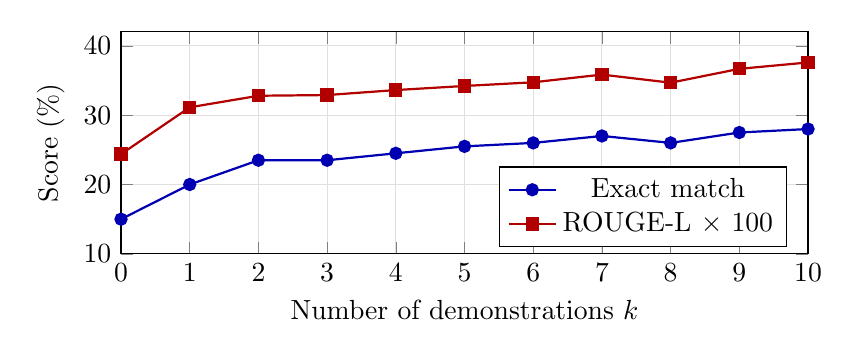
\begin{tikzpicture}
    \begin{axis}[width=0.85\columnwidth, height=4.4cm, xlabel={Number of demonstrations $k$},
      ylabel={Score (\%)}, xmin=0, xmax=10, ymin=10, ymax=42, xtick={0,1,...,10},
      legend pos=south east, grid=major, grid style={gray!25}, every axis plot/.append style={thick}]
      \addplot[mark=*, color=blue!70!black] coordinates {(0,15)(1,20)(2,23.5)(3,23.5)(4,24.5)(5,25.5)(6,26)(7,27)(8,26)(9,27.5)(10,28)};
      \addlegendentry{Exact match}
      \addplot[mark=square*, color=red!70!black] coordinates {(0,24.38)(1,31.13)(2,32.80)(3,32.90)(4,33.62)(5,34.21)(6,34.74)(7,35.85)(8,34.68)(9,36.68)(10,37.60)};
      \addlegendentry{ROUGE-L $\times$ 100}
    \end{axis}
  \end{tikzpicture}
  \caption{Exact match and ROUGE-L of the frozen baseline against the number of demonstrations (200 queries).}
  \label{fig:shots}
\end{figure}

\subsection{Qwen2-1.5B: Adapter Placement and Rank}\label{sec:qwen}

The rank sweeps are not all equal in density: $q,k,v,o$ was run at four ranks, whereas $q,v$ and all-linear were run at two ranks each, due to time limitations, and $q,v$ was not explored further, as it did not yield good results in the other experiments.

All eight runs lie between 84.13\% and 86.62\%. The four runs $q,k,v,o$ at $r=4$ and $r=8$ and $q,v$ at $r=8$ and $r=16$ span 86.06\% to 86.62\%, i.e.\ 0.56 points. The $q,v$ run at $r=8$ has the same number of trainable parameters as the best run (5,816,320), and is 0.48 points lower. These differences are small compared to the resolution of a single seed and a 73-image test set, and the runs are not ranked here.

The four remaining runs ($q,k,v,o$ $r=32$, all-linear $r=16$ and $r=8$, and $q,k,v,o$ $r=16$) are about 0.9 to 2.5 points below the best run. Larger trainable counts did not yield higher exact match: the three runs with the highest number of trainable parameters (23.2, 14.0 and 13.4 million) score 85.74\%, 84.85\% and 85.50\% respectively, which is lower than the four runs with 5.8 to 6.9 million. These 5.8 to 6.9 million parameters include the projectors and modality embeddings in each run, accounting for 81\% of the total trainable parameters in the smallest configuration.

Each of the runs was terminated by early stopping after 10 to 15 epochs (out of 100). The lowest validation loss (0.1159) is not the loss of the best test run (the best run, $q,k,v,o$ $r=4$, has 0.1236). Only the checkpoint with minimum validation loss of each run was used for testing. The minimum validation loss against the test EM for the 16 runs is plotted in Fig.~\ref{fig:valloss}.

\begin{figure}[!t]
  \centering
  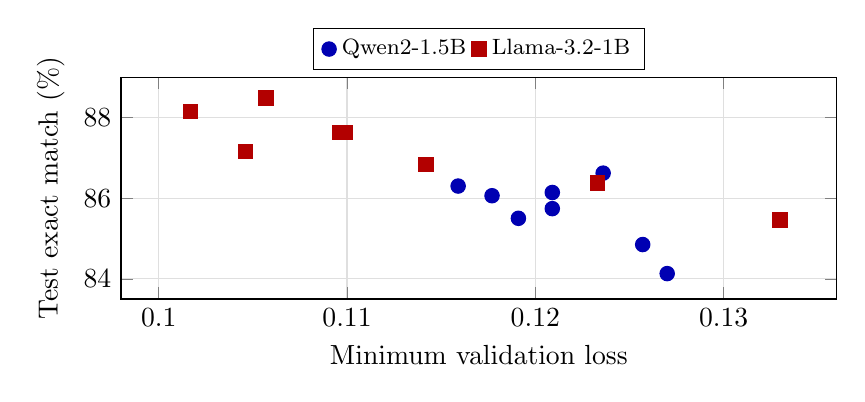
\begin{tikzpicture}
    \begin{axis}[width=0.88\columnwidth, height=4.4cm, xlabel={Minimum validation loss},
      ylabel={Test exact match (\%)}, grid=major, grid style={gray!25},
      legend style={at={(0.5,1.03)}, anchor=south, legend columns=2, font=\footnotesize}, xmin=0.098, xmax=0.136, ymin=83.5, ymax=89, scaled x ticks=false, xtick={0.10,0.11,0.12,0.13}, x tick label style={/pgf/number format/fixed, /pgf/number format/precision=2}]
      \addplot[only marks, mark=*, mark size=2.6pt, color=blue!70!black] coordinates
        {(0.1236,86.62)(0.1159,86.30)(0.1209,86.14)(0.1177,86.06)(0.1209,85.74)(0.1191,85.50)(0.1257,84.85)(0.1270,84.13)};
      \addlegendentry{Qwen2-1.5B}
      \addplot[only marks, mark=square*, mark size=2.6pt, color=red!70!black] coordinates
        {(0.1057,88.48)(0.1017,88.15)(0.1096,87.63)(0.1099,87.63)(0.1046,87.15)(0.1142,86.83)(0.1233,86.38)(0.1330,85.46)};
      \addlegendentry{Llama-3.2-1B}
    \end{axis}
  \end{tikzpicture}
  \caption{Minimum validation loss against test exact match for the 16 runs. Within each backbone the lowest validation loss is not the run with the highest exact match.}
  \label{fig:valloss}
\end{figure}

\subsection{Llama-3.2-1B Backbone}\label{sec:llama}

Exact match ranges from 85.46\% (all-linear, $r=16$) to 88.48\% ($q,k,v,o$, $r=8$).

Llama outperforms Qwen2 on 7 of 8 pairs at the same placement and rank, with margins from $+0.24$ to $+4.03$ points. As with Qwen2, the lowest validation loss (0.1017, $q,k,v,o$ $r=16$) is not associated with the highest EM.

\subsection{Question Categories}

The six categories have 584, 584, 292, 438, 292 and 292 rows, i.e.\ 8, 8, 4, 6, 4 and 4 questions for each of the 73 images, so one image contributes 4 rows (1.4 points) to a cell of 292 rows. The percentages are an exact reproduction of the integer counts -- 2150, 2088, 2144 and 2196 -- that add up to the total number of correct answers for each run.

Presence and detection have the highest EM (90.75\% to 95.21\%) while localization and direction have the lowest (71.23\% to 79.45\%). The 62 additional correct rows of $q,k,v,o$ $r=4$ over $r=16$ are concentrated in two categories: 28 for cross-modal reasoning (85.96\% compared to 76.37\%) and 24 for localization and direction (79.45\% compared to 71.23\%); the other four categories add 10 overall, and flight planning and classification favour $r=16$. In four of six categories (presence and detection, flight planning, classification, cross-modal reasoning) Llama $q,k,v,o$ $r=8$ has the highest value among the four runs compared. No error analysis was performed, and it is not determined why some categories are more difficult than others. The differences are only a few points on 292-row cells and 73 images in one run and should not be interpreted as stable differences.

\subsection{Threats to Validity}

\begin{enumerate}[leftmargin=*, itemsep=1pt, topsep=2pt, parsep=0pt]
  \item \textbf{Single seed and small test set.} Each configuration is trained once, and the test set contains 73 images.
  \item \textbf{Uncontrolled backbone comparison.} The Qwen2 and Llama runs, and some runs within each backbone, differ in learning rate, number of planned epochs, early-stopping conditions and batch layout (Section~\ref{sec:llama}).
\end{enumerate}

\section{Conclusion and Future Scope}

\subsection{Conclusion}

On the 2,482 test rows, the Qwen2-1.5B runs reach 84.13\% to 86.62\% exact match with 5.8 to 23.2 million trainable parameters, and the Llama-3.2-1B runs reach 85.46\% to 88.48\%. For Qwen2, $q,k,v,o$ at $r=4$ (86.62\%) and $q,v$ at $r=8$ (86.14\%) have the same 5,816,320 trainable parameters, and four attention-only configurations differ by only 0.56 points, which is less than the variation expected from a single seed and 73 test images. No higher exact match was obtained with the larger adapters. For Llama, comparisons by rank or placement cannot be made reliably, since learning rate, epochs, early-stopping settings and batch layout differ from run to run. The same holds for the comparison of the two backbones. A frozen Qwen2.5-VL-3B model with 0 to 10 demonstrations achieves 15.00\% to 28.00\% exact match on 200 sampled queries, which serves only as a reference, as the queries are not paired with the fine-tuning split.

\subsection{Future Scope}

\begin{itemize}[leftmargin=*, itemsep=1pt, topsep=2pt, parsep=0pt]
  \item For each configuration, run several seeds to test for differences of approximately one point, and run the bootstrap across all the runs.
  \item Retrain the two backbones with the same learning rate, schedule, early-stopping parameters and batch layout to separate backbone and adapter effects.
  \item Rerun the frozen baseline on the 73-image test split (one image key per query) with the audited image pairing.
\end{itemize}


\begin{thebibliography}{00}
\bibitem{wildfirevqa}
M. Habibpour, N. Alipour Talemi, J. Spodnik, C. J. Khoury, F. Afghah, ``WildFireVQA: A
Large-Scale Radiometric Thermal VQA Benchmark for Aerial Wildfire Monitoring'',
arXiv:2604.20190, 2026. Data and code: \url{https://github.com/mobiiin/WildFire_VQA}.
\bibitem{flame3}
B. Hopkins, L. ONeill, M. Marinaccio, E. Rowell, R. Parsons, S. Flanary, I. Nazim,
C. Seielstad, F. Afghah, ``FLAME 3 Dataset: Unleashing the Power of Radiometric Thermal
UAV Imagery for Wildfire Management'', arXiv:2412.02831, 2024.
\bibitem{brown2020}
T. Brown \textit{et al.}, ``Language Models are Few-Shot Learners'', Advances in
Neural Information Processing Systems (NeurIPS), Vol. 33, pp. 1877-1901, 2020.
\bibitem{bai2025}
S. Bai \textit{et al.}, ``Qwen2.5-VL Technical Report'', arXiv:2502.13923, 2025.
\bibitem{radford2021}
A. Radford \textit{et al.}, ``Learning Transferable Visual Models From Natural
Language Supervision'', Proceedings of the 38th International Conference on Machine
Learning (ICML), PMLR 139, pp. 8748-8763, 2021.
\bibitem{dettmers2023}
T. Dettmers, A. Pagnoni, A. Holtzman, L. Zettlemoyer, ``QLoRA: Efficient
Finetuning of Quantized LLMs'', Advances in Neural Information Processing
Systems (NeurIPS), Vol. 36, 2023.
\bibitem{hu2022}
E. J. Hu \textit{et al.}, ``LoRA: Low-Rank Adaptation of Large Language Models'',
International Conference on Learning Representations (ICLR), 2022.
\bibitem{qwen2}
A. Yang \textit{et al.}, ``Qwen2 Technical Report'', arXiv:2407.10671, 2024.
\bibitem{mithan}
MIT HAN Lab, ``Qwen2-VL-1.5B-Instruct'', Hugging Face model repository, \url{https://huggingface.co/mit-han-lab/Qwen2-VL-1.5B-Instruct}.
\bibitem{llama32}
Meta AI, ``Llama-3.2-1B-Instruct'', Hugging Face model repository, \url{https://huggingface.co/meta-llama/Llama-3.2-1B-Instruct}.
\bibitem{peft2024survey}
``Parameter-Efficient Fine-Tuning for Vision-Language Models: The Post-Transformer Evolution'',
arXiv preprint, 2024.
\bibitem{ak2024aligning}
K. E. Ak, J. Mohta, D. Dimitriadis, S. Manchanda, Y. Xu, M. Shen,
``Aligning Vision Language Models with Contrastive Learning'',
Proceedings of the European Conference on Computer Vision (ECCV) Workshops,
Lecture Notes in Computer Science, Vol. 15640, pp. 32-45, 2025.
\bibitem{vlpet2024}
Z.-Y. Hu, Y. Li, M. R. Lyu, L. Wang, ``VL-PET: Vision-and-Language Parameter-Efficient
Tuning via Granularity Control'', Proceedings of the IEEE/CVF International Conference on
Computer Vision (ICCV), 2023. arXiv:2308.09804.
\bibitem{remotesensing2024}
X. Weng, C. Pang, G.-S. Xia, ``Vision-Language Modeling Meets Remote Sensing: Models,
Datasets, and Perspectives'', arXiv preprint, 2025.
\bibitem{molmo2024}
M. Deitke \textit{et al.}, ``Molmo and PixMo: Open Weights and Open Data for
State-of-the-Art Vision-Language Models'', arXiv:2409.17146, 2024.
\bibitem{visioncore2024}
``VisionCore: Adapting Efficient Visual Answering Through Enhanced Spatial Reasoning'',
arXiv preprint, 2024.
\bibitem{synthvlm2024}
Z. Liu \textit{et al.}, ``SynthVLM: Towards High-Quality and Efficient Synthesis of
Image-Caption Datasets for Vision-Language Models'', arXiv:2407.20756, 2024.
\end{thebibliography}

\end{document}
